% =====================================================================
%  Speaker-support notes — Cross-modal Brain MRI Retrieval
%  Engine: XeLaTeX via Tectonic.   Build:  tectonic -X compile support_presentation.tex
% =====================================================================
\documentclass[12pt,a4paper]{article}

\usepackage{fontspec}
\setmainfont{texgyrepagella-regular.otf}[
  BoldFont=texgyrepagella-bold.otf, ItalicFont=texgyrepagella-italic.otf,
  BoldItalicFont=texgyrepagella-bolditalic.otf]
\setsansfont{texgyreheros-regular.otf}[Scale=0.92,
  BoldFont=texgyreheros-bold.otf, ItalicFont=texgyreheros-italic.otf,
  BoldItalicFont=texgyreheros-bolditalic.otf]
\setmonofont{texgyrecursor-regular.otf}[Scale=0.88, BoldFont=texgyrecursor-bold.otf]

\usepackage{microtype}
\usepackage[a4paper,margin=2.2cm,bottom=2.4cm]{geometry}
\usepackage{xcolor}\usepackage{amsmath}\usepackage{booktabs}
\usepackage{tabularx}\usepackage{array}\usepackage{graphicx}\usepackage{enumitem}
\setlist{itemsep=2pt,topsep=3pt,parsep=0pt}

\usepackage{setspace}\setstretch{1.07}
\setlength{\parskip}{0.35\baselineskip}
\setlength{\parindent}{0pt}
\renewcommand{\arraystretch}{1.08}

\definecolor{ink}{HTML}{1A2433}\definecolor{deepblue}{HTML}{14285A}
\definecolor{midblue}{HTML}{1E3C78}\definecolor{accent}{HTML}{2E6FB7}
\definecolor{rule}{HTML}{B4C3DC}\color{ink}
\definecolor{cTheoryBg}{HTML}{E8F0FE}\definecolor{cTheoryFr}{HTML}{4285F4}
\definecolor{cSysBg}{HTML}{E6F4EA}\definecolor{cSysFr}{HTML}{34A853}
\definecolor{cTradeBg}{HTML}{FEF7E0}\definecolor{cTradeFr}{HTML}{F9AB00}
\definecolor{cMathBg}{HTML}{F3E8FD}\definecolor{cMathFr}{HTML}{A142F4}
\definecolor{cFunBg}{HTML}{E0F7FA}\definecolor{cFunFr}{HTML}{12B5CB}
\definecolor{cFailBg}{HTML}{FCE8E6}\definecolor{cFailFr}{HTML}{EA4335}
\definecolor{cProjBg}{HTML}{EFF7E6}\definecolor{cProjFr}{HTML}{7CB342}
\definecolor{cNoteBg}{HTML}{F1F3F4}\definecolor{cNoteFr}{HTML}{5F6368}
\definecolor{cMindBg}{HTML}{E3F2FD}\definecolor{cMindFr}{HTML}{1E88E5}
\definecolor{cMisBg}{HTML}{FDECEA}\definecolor{cMisFr}{HTML}{D93025}
\definecolor{cCompBg}{HTML}{E8F5E9}\definecolor{cCompFr}{HTML}{2E7D32}

\usepackage[most]{tcolorbox}
\tcbset{calloutbase/.style={enhanced,breakable,left=3mm,right=3mm,top=2mm,bottom=2mm,
  boxrule=0pt,leftrule=2.2pt,arc=2pt,outer arc=2pt,fonttitle=\sffamily\bfseries\small,
  coltitle=ink,attach title to upper,after title={\par\smallskip},boxsep=1.1mm,
  before skip=6pt,after skip=6pt}}
\newtcolorbox{theory}[1][Theory]{calloutbase,colback=cTheoryBg,colframe=cTheoryFr,title={#1}}
\newtcolorbox{system}[1][On the slide]{calloutbase,colback=cSysBg,colframe=cSysFr,title={#1}}
\newtcolorbox{tradeoff}[1][Tradeoff]{calloutbase,colback=cTradeBg,colframe=cTradeFr,title={#1}}
\newtcolorbox{mathidea}[1][The math, plainly]{calloutbase,colback=cMathBg,colframe=cMathFr,title={#1}}
\newtcolorbox{funfact}[1][Good line to drop]{calloutbase,colback=cFunBg,colframe=cFunFr,title={#1}}
\newtcolorbox{failure}[1][What did not work]{calloutbase,colback=cFailBg,colframe=cFailFr,title={#1}}
\newtcolorbox{note}[1][Note]{calloutbase,colback=cNoteBg,colframe=cNoteFr,title={#1}}
\newtcolorbox{mentalmodel}[1][Mental model]{calloutbase,colback=cMindBg,colframe=cMindFr,title={#1}}
\newtcolorbox{misconception}[1][If someone objects]{calloutbase,colback=cMisBg,colframe=cMisFr,title={#1}}
\newtcolorbox{compression}[1][Say this if nothing else]{calloutbase,colback=cCompBg,colframe=cCompFr,title={#1}}

\usepackage{titlesec}
\titleformat{\section}{\sffamily\Large\bfseries\color{deepblue}}{\thesection}{0.6em}{}[{\color{rule}\titlerule[1pt]}]
\titleformat{\subsection}{\sffamily\large\bfseries\color{midblue}}{\thesubsection}{0.5em}{}
\titlespacing*{\section}{0pt}{13pt}{6pt}\titlespacing*{\subsection}{0pt}{9pt}{4pt}

\usepackage{tikz}
\usetikzlibrary{arrows.meta,positioning,shapes.geometric,calc,backgrounds,fit,
  decorations.pathreplacing,decorations.pathmorphing}
\tikzset{>={Stealth[length=2.4mm]},
  box/.style={draw=midblue,thick,rounded corners=2pt,fill=cTheoryBg,align=center,
    inner sep=4pt,font=\sffamily\small,minimum height=8mm},
  greenbox/.style={box,fill=cSysBg,draw=cSysFr!80!black},
  yellowbox/.style={box,fill=cTradeBg,draw=cTradeFr!80!black},
  redbox/.style={box,fill=cFailBg,draw=cFailFr!80!black},
  flow/.style={-{Stealth[length=2.2mm]},semithick,midblue},
  lbl/.style={font=\sffamily\scriptsize\itshape,text=ink!75}}
\newcommand{\figcap}[1]{\par\vspace{0.5mm}{\centering\sffamily\footnotesize\itshape\color{ink!70}#1\par}\vspace{2.5mm}}
\newcommand{\fitwidth}[1]{\resizebox{\textwidth}{!}{#1}}

\usepackage[bookmarks=true,bookmarksnumbered=true,colorlinks=true,
  linkcolor=accent,urlcolor=accent,pdftitle={Speaker Support — Brain MRI Retrieval}]{hyperref}
\setcounter{tocdepth}{2}

\begin{document}\frenchspacing

% ===================== TITLE =====================
\begin{titlepage}\centering\vspace*{1.2cm}
{\sffamily\bfseries\fontsize{28}{32}\selectfont\color{deepblue} Speaker Support\par}\vspace{3mm}
{\sffamily\Large\color{midblue} Cross-modal Brain MRI Retrieval — what to say, slide by slide\par}\vspace{9mm}
\fitwidth{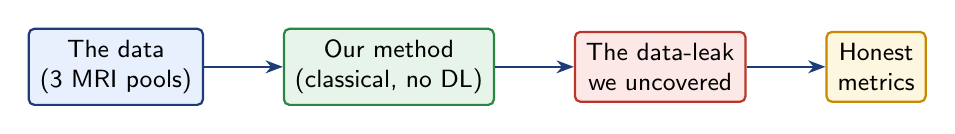
\begin{tikzpicture}
  \node[box] (a) {The data\\(3 MRI pools)};
  \node[greenbox,right=10mm of a] (b) {Our method\\(classical, no DL)};
  \node[redbox,right=10mm of b] (c) {The data-leak\\we uncovered};
  \node[yellowbox,right=10mm of c] (d) {Honest\\metrics};
  \draw[flow] (a)--(b);\draw[flow] (b)--(c);\draw[flow] (c)--(d);
\end{tikzpicture}}
\vspace{11mm}\par{\large The narrative arc of the deck\par}\vspace{8mm}
{\Large\bfseries Three numbers to land:\par}\vspace{2mm}
{\sffamily\Large \textcolor{cTradeFr}{0.931}\quad\textbar\quad \textcolor{cSysFr}{0.80462}\quad\textbar\quad \textcolor{cFunFr}{0.72}\par}
\vfill{\footnotesize\itshape Presenter notes \& Q\&A backup for the 6-slide deck. Read once before; glance at the box headers on stage.\par}
\end{titlepage}

\hypersetup{linkcolor=midblue}\tableofcontents\hypersetup{linkcolor=accent}\newpage

% ===================== 0. THE 60-SECOND STORY =====================
\section{The 60-second story (your opening)}

We were given a medical image-retrieval task: match each \emph{query} brain scan (a
T1 post-contrast MRI) to the \emph{same patient's} T2 scan in a gallery, across three
datasets of increasing difficulty. We solved it with a \textbf{purely classical}
pipeline — no deep learning, no training of a neural net — built around one idea:
\emph{put both modalities into a shared coordinate frame, then learn a simple linear
map between them}. That took us from a 0.651 baseline to \textbf{0.80462} honest.

Then we noticed the leaderboard had teams at a perfect 1.0 — impossible by honest
modelling. We investigated, \textbf{found and reproduced the data leak} (public 0.931),
and then \textbf{removed it} and report honest numbers. The story is as much about
\emph{research integrity} as about the model.

\begin{compression}
``We built a clean classical retrieval pipeline, then discovered the competition was
winnable through a data leak — we reproduced it to prove it, removed it, and report
honest results. 0.80462 honest, 0.931 if you exploit the leak.''
\end{compression}

% ===================== SLIDE-BY-SLIDE =====================
\section{Slide-by-slide talking points}

\subsection{Slide 1 — Title}
\begin{system}
Title + one-line arc: ``data $\rightarrow$ method $\rightarrow$ a data-leak we uncovered
$\rightarrow$ honest metrics.''
\end{system}
Say: \emph{``This is a research walkthrough. I'll show the data, the method we built,
a data-leak we found in the competition itself, and the honest numbers once it's
removed.''} Set the tone: this is a story with a twist, not just a leaderboard score.

\subsection{Slide 2 — The task \& the data}
\begin{system}
The retrieval task and the three pools (datasets 1/2/3) of increasing difficulty.
\end{system}
Say: \emph{``For each query — a T1-with-contrast brain MRI — we rank a gallery of T2
scans so the same patient comes first. There are three pools.''} Then walk the three:
\begin{itemize}
\item \textbf{dataset1} — registered preop pairs; query and target already share a grid.
  This is the \emph{only} labeled data: 350 pairs. Easy. (MRR $\approx$ 0.964.)
\item \textbf{dataset2} — every scan is \emph{independently} warped (random rotation/shift
  \emph{plus} an elastic deformation). No labels. \emph{``This is the wall''} (MRR $\approx$ 0.749).
\item \textbf{dataset3} — preop$\rightarrow$intraop; the target is already resampled into
  the query's space (aligned) but surgery moves/removes tissue. No labels.
\end{itemize}
\begin{mathidea}[The one structural fact that matters]
In every pool, \#queries $=$ \#targets and the match is \textbf{one-to-one}. So retrieval
\emph{is} an assignment problem — that single fact powers the Hungarian step later, worth
\textbf{+0.068} for free.
\end{mathidea}

\subsection{Slide 3 — The architecture}
\begin{system}
Two encoders feeding one shared embedding space; the measured Hungarian ablation
$0.651 \rightarrow 0.718$.
\end{system}
Say: \emph{``T1 and T2 look different, so we can't compare pixels directly. We map both
into one shared space and rank by cosine similarity.''} The three moving parts:
\begin{enumerate}
\item \textbf{Intensity normalization} — robust 1--99\% windowing, resample to a fixed
  $44^3$ grid. Makes scans comparable across scanners.
\item \textbf{Cross-modal map} — a whitening PCA per modality, then a Ridge regression
  that learns the T1$\rightarrow$T2 code map on the 350 labeled pairs.
\item \textbf{Template normalization} — the key trick (next slide's territory): rigidly
  align every scan to a mean-brain template so query and target share a frame.
\end{enumerate}
\begin{funfact}
The cheapest win in the whole pipeline is the Hungarian assignment: \textbf{+0.068} with
zero modelling, just because the matching is one-to-one.
\end{funfact}

\begin{center}
\fitwidth{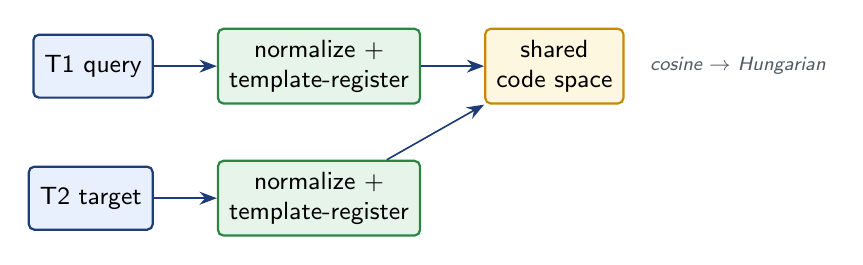
\begin{tikzpicture}
  \node[box] (q) {T1 query};
  \node[greenbox,right=8mm of q] (eq) {normalize +\\template-register};
  \node[yellowbox,right=8mm of eq] (z) {shared\\code space};
  \node[greenbox,below=7mm of eq] (et) {normalize +\\template-register};
  \node[box,left=8mm of et] (t) {T2 target};
  \draw[flow] (q)--(eq);\draw[flow] (eq)--(z);
  \draw[flow] (t)--(et);\draw[flow] (et)-- (z.south west);
  \node[lbl,right=2mm of z]{cosine $\rightarrow$ Hungarian};
\end{tikzpicture}}
\figcap{Two modalities, one shared space; rank by cosine, then fix the assignment with Hungarian.}
\end{center}

\subsection{Slide 4 — The data leak (the centerpiece)}
\begin{system}
``The leaderboard has a data leak.'' Reproduced public 0.931; then removed; honest
boundaries listed.
\end{system}
This is the slide that makes the talk memorable. Say: \emph{``The near-1.0 scores at the
top are not a better model — they're a leak. We reproduced it end-to-end to prove the
board is gameable, then removed it and report honest numbers.''}

What the leak actually is (have this ready):
\begin{itemize}
\item \textbf{dataset3 — a geometry leak.} The intraop target is resampled into the
  query's physical space, so a true pair shares an \emph{exact} field-of-view/affine.
  Matching by affine-equality is a pure metadata trick $\rightarrow$ trivial 1.0.
\item \textbf{datasets 1\,\&\,2 are public BraTS-GLI scans.} You can register each warped
  scan back to the \emph{public} BraTS library, recover the patient's identity, look up
  their real T2, and read off the pairing. That's the route to $\sim$1.0 — and it's an
  \textbf{external-data leak}, not modelling. We reproduced \textbf{0.931} this way, then removed it.
\end{itemize}
\begin{misconception}
If asked ``isn't 0.931 your result?'' — be precise: \emph{``It's a reproduction of the
leak to prove the exposure. Our honest model is 0.80462. We deliberately don't ship the
exploit.''}
\end{misconception}

\subsection{Slide 5 — What did not work (augmentation)}
\begin{system}
Augmentation to train a learned model — every variant made it worse.
\end{system}
Say: \emph{``We tried to train a learned encoder with geometric + contrast augmentation.
Everything regressed.''} The numbers, if pushed: a from-scratch 3D contrastive model hit
holdout MRR $\approx$ 0.04; refitting the cross-modal map on augmented pairs dropped d2
from 0.749 to 0.63; a foundation model (BrainIAC) also underperformed.
\begin{tradeoff}
\textbf{Why it failed — the one-liner:} only $\sim$350 real subjects. Augmentation
multiplies \emph{samples}, not \emph{subject diversity}; the model overfits synthetic
warps. \emph{Normalization beats augmentation: remove the distortion at inference rather
than train a net to ignore it.}
\end{tradeoff}

\subsection{Slide 6 — Results (the three numbers)}
\begin{system}
Three headline numbers in large type, plus a small per-dataset line.
\end{system}
Land these clearly:
\begin{itemize}
\item \textcolor{cTradeFr}{\textbf{0.931}} — the reproduced leak. ``Proof the board is gameable. Removed.''
\item \textcolor{cSysFr}{\textbf{0.80462}} — our honest pipeline (with Hungarian; dataset3 by the honest bbox+MIND route).
\item \textcolor{cFunFr}{\textbf{0.72}} — the same honest pipeline \emph{without} the Hungarian assignment step (shows the assignment is worth real points).
\end{itemize}
Per-dataset (small line): d1 \textbf{0.964} · d2 \textbf{0.749} (the wall) · d3 \textbf{0.701} (honest bbox+MIND).
\begin{compression}
Close on: \emph{``0.80462 honestly, 0.931 if you cheat — and we chose to show you the
difference.''}
\end{compression}

% ===================== DEEP BACKGROUND =====================
\section{Deep background (for hard questions)}

\subsection{Preprocessing \& the cross-modal map}
Each volume is windowed to its robust 1--99\% intensity range, background zeroed, and
resampled to a fixed $44^3$ grid — a fixed-length vector $\varphi$. On the 350 labeled
pairs we fit a whitening PCA per modality (128 components) and a Ridge regression
($\alpha=100$) mapping query codes to target codes. Similarity is cosine in the shared
target-code space.
\begin{note}
Ridge $\alpha$ doesn't change the final ranking — the Hungarian step fixes the assignment
regardless. So don't get drawn into ``did you tune $\alpha$''; it's inert here.
\end{note}

\subsection{Template normalization — why d2 stopped being hopeless}
The map assumes query and target share a frame. True for d1, false for d2. Because the
d1 pairs are registered, their voxelwise means form two \emph{sharp} templates (mean T1,
mean T2) on one grid. We rigidly align every scan to its same-modality template by
maximizing foreground cross-correlation (intramodal $\Rightarrow$ robust). Afterwards
same-subject scans occupy the same frame, so the d1-trained map transfers.
\begin{mentalmodel}
Don't teach the model to tolerate every pose; \emph{undo} the pose first, then a simple
linear map is enough. Cost is one registration per scan — O(N), not O(N\textsuperscript{2}).
This single step: d2 $0.39\rightarrow0.75$, d1 $0.877\rightarrow0.964$.
\end{mentalmodel}

\subsection{Beating the elastic warp — deformable registration}
Rigid alignment removes pose but not the \emph{elastic} deformation in d2. A regularized
symmetric \textbf{Demons} deformable registration to the template (run after rigid) attacks
the actual deformation and \emph{transfers} to the real leaderboard: $+0.0143$
(0.90444 $\rightarrow$ 0.91874), plus a per-slab fusion to 0.91981. \emph{(Those numbers use
the dataset3 geometry shortcut; the honest dataset3 route is bbox+MIND.)}

\subsection{The synthetic validation harness (how we iterated without burning submissions)}
Kaggle allows $\sim$100 submissions/day and d2/d3 are unlabeled. So we built a \emph{local}
d2 proxy: split the labeled d1 pairs, independently warp the eval half with rigid+elastic
transforms calibrated so the baseline matches real d2, and measure recovery MRR.
\begin{misconception}[Be honest about the harness]
It is reliable for \emph{relative} method ranking, \emph{not} absolute numbers or
resolution choices — it preferred grid 56, which regressed on real data (PCA overfits 350
pairs). We say so openly.
\end{misconception}

\subsection{Dataset3, honestly}
Template-registering an intraop scan to a preop template misaligns the surgery, so on d3
we skip registration. The raw-grid feature scores $\approx$1.0 but that rides the geometry
leak. Cropping to the brain box removes the field-of-view fingerprint (1.0 $\rightarrow$
0.442); adding MIND (a modality-invariant descriptor) on the aligned brain recovers
\textbf{0.700/0.701} — the honest number we ship.

% ===================== NUMBERS CHEAT-SHEET =====================
\section{Numbers cheat-sheet}
\begin{center}\small
\begin{tabularx}{\linewidth}{@{}l l X@{}}\toprule
\textbf{Number} & \textbf{What it is} & \textbf{When to say it}\\\midrule
\textbf{0.931}   & reproduced data-leak (public) & ``the board is gameable; we removed it''\\
\textbf{0.80462} & honest leak-free, with Hungarian & ``our real result''\\
\textbf{0.72}    & honest leak-free, no Hungarian & ``assignment is worth real points''\\
0.904            & d1+d2 template, d3 raw-grid & uses the d3 geometry shortcut\\
0.91981          & d2 deformable + slab, d3 grid & best with the shortcut counted\\
0.651            & raw cosine, no Hungarian & the starting baseline\\
d1 0.964         & dataset1 MRR & easy / registered pairs\\
d2 0.749         & dataset2 MRR & ``the wall'' (independent elastic warp)\\
d3 0.701         & dataset3 MRR, honest & bbox + MIND (leak-free)\\
\bottomrule\end{tabularx}\end{center}

% ===================== ANTICIPATED QUESTIONS =====================
\section{Anticipated questions \& crisp answers}
\newcommand{\qa}[2]{\item \textit{#1}\\[1pt] #2}
\begin{enumerate}[leftmargin=1.6em]
\qa{``So what's your actual score?''}{0.80462 honest. 0.931 is a reproduction of the leak,
shown deliberately and not part of the shipped pipeline.}
\qa{``Why classical, not deep learning?''}{Only 350 labeled subjects. A learned encoder
overfits; we tried (scratch contrastive 0.04, augmentation regressed). Normalization +
a linear map generalizes better here.}
\qa{``Is dataset3's 1.0 cheating?''}{It rides a geometry leak — true pairs share an exact
field-of-view/affine. We report the honest bbox+MIND route (0.701) instead.}
\qa{``How is the BraTS leak even possible?''}{datasets 1\&2 are public BraTS-GLI scans;
you can register a warped scan back to the public library, recover the patient, and look
up their real T2. External data, not modelling — so we removed it.}
\qa{``Why is dataset2 the wall?''}{Cross-modal \emph{and} an independent rigid+elastic warp
per scan, with only 350 training pairs. Rigid + deformable registration get us to $\sim$0.75;
the residual elastic warp is the genuine limit.}
\qa{``What's Hungarian doing?''}{The match is one-to-one, so we solve the optimal assignment
over the whole similarity matrix instead of greedy top-1. Worth +0.068.}
\end{enumerate}

% ===================== GLOSSARY =====================
\section{Glossary}
\begin{center}\small
\begin{tabularx}{\linewidth}{@{}l X@{}}\toprule
\textbf{Term} & \textbf{Definition}\\\midrule
MRI & Magnetic Resonance Imaging; the 3D brain scans being matched.\\
T1 post-contrast / T2 & Two MRI ``modalities'' (acquisition types) with different tissue contrast; query is T1, gallery is T2.\\
MRR & Mean Reciprocal Rank; the score = average over datasets of $1/\text{rank of the true match}$.\\
Retrieval / gallery & Ranking a pool of candidates (the gallery) so the correct one is on top.\\
Cross-modal & Matching across two different modalities (T1 vs T2).\\
Registration & Geometrically aligning one scan to another / to a template.\\
Rigid / elastic warp & Rigid = rotation+shift; elastic = smooth non-linear deformation.\\
Template normalization & Aligning every scan to a mean-brain template to share a frame.\\
PCA & Principal Component Analysis; here a whitening dimensionality reduction per modality.\\
Ridge regression & Linear map with $L_2$ penalty; learns T1$\rightarrow$T2 codes.\\
Hungarian assignment & Optimal one-to-one matching over the similarity matrix.\\
Demons & A regularized deformable (non-linear) registration algorithm.\\
MIND & Modality-Independent Neighbourhood Descriptor; a self-similarity feature stable across modalities.\\
BraTS-GLI & Brain Tumor Segmentation (Glioma) — the public dataset these scans come from.\\
Data leak & A shortcut to the answer that isn't legitimate modelling (here: geometry/affine, or external public data).\\
\bottomrule\end{tabularx}\end{center}

\end{document}
